\chapter{Implementacija i korisničko sučelje}
		
		
		\section{Korištene tehnologije i alati}
			
		Komunikacija u timu realizirana je korištenjem aplikacije WhatsApp\footnote{\url{https://www.whatsapp.com/}}. Za izradu UML dijagrama primarno je korišten alat Astah UML\footnote{\url{http://astah.net/editions/community}}, no za određene dijagrame je radi preglednosti i oku ugodnijeg dizajna korišten \textit{plugin} PlantUML\footnote{\url{https://plantuml.com/}} za IntelliJ radnu okolinu. Za upravljanje izvornim kodom i njegovim inačicama koristili smo Git\footnote{\url{https://git-scm.com/}}. Udaljeni repozitorij projekta u kojem se nalazi cjelokupni izvorni kod dostupan je na web platformi GitLab\footnote{\url{https://gitlab.com/}}.
			
				Kao razvojno okruženje korišteni su IntelliJ\footnote{\url{https://www.jetbrains.com/idea/}} - integrirano razvojno okruženje (IDE) tvrtke JetBrains, i Eclipse\footnote{\url{https://www.eclipse.org/}} - IDE tvrtke The Eclipse Foundation. IDE se koristi za razvoj web-stranica, web-aplikacija, web-usluga te mobilnih aplikacija. IDE pruža integraciju s drugim alatima za razvoj kao što je primjerice Maven\footnote{\url{https://maven.apache.org/}} kojeg smo koristili za lokalno upravljanje projektom, uključivanje raznih biblioteka o kojima aplikacija ovisi, te automatiziranu izgradnju projekta i pakiranje u JAR arhivu. Oba IDE-a podržavaju sustave kontrole verzioniranja kao što je Git.
				
				Aplikacija je napisana koristeći radni okvir Spring\footnote{\url{https://spring.io/}} i jezik Java\footnote{\url{https://www.java.com/en/}} za izradu \textit{backenda} te Bootstrap\footnote{\url{https://getbootstrap.com/}} i jezik JavaScript\footnote{\url{https://www.javascript.com/}} za izradu \textit{frontenda}.
 			
			\eject 
		
	
		\section{Ispitivanje programskog rješenja}
			
			\subsection{Ispitivanje komponenti}
		
			
			\subsection{Ispitivanje sustava}
			
			\eject 
		
		
		\section{Dijagram razmještaja}
			
			Dijagrami razmještaja opisuju topologiju sklopovlja i programsku potporu koja se koristi u implementaciji sustava u njegovom radnom okruženju. Na poslužiteljskom računalu se nalaze web poslužitelj i poslužitelj baze podataka. Klijenti koriste web preglednik kako bi pristupili web aplikaciji. Sustav je baziran na arhitekturi ”klijent – poslužitelj”, a komunikacija između računala korisnika (klijent, zaposlenik, vlasnik, administrator) i poslužitelja odvija se preko HTTPS veze.
			
			\begin{figure}[H]
					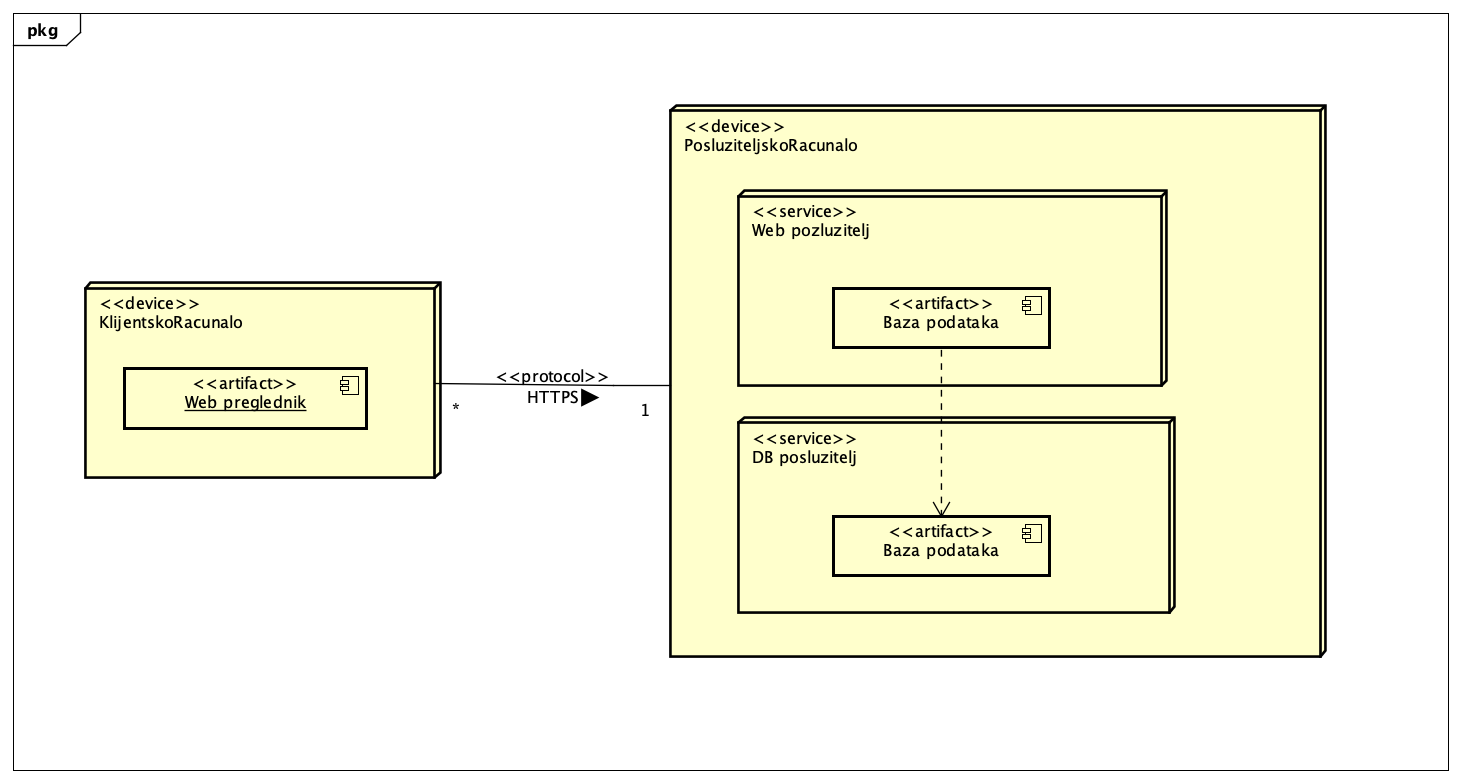
\includegraphics[scale=0.4]{figures/Deployment Diagram0.PNG}
					\centering
					\caption{Dijagram razmještaja}
					\label{fig:Dijagram razmještaja}
				\end{figure}
			\eject 
		
		\section{Upute za puštanje u pogon}
		
		\noindent {\textbf{Mikroservisi i Docker}}
	
		
		Sustav je razvijen idejom mikroservisne arhitekture. Svaki dio aplikacije je napravljen kao poseban servis koji može raditi na jednom ili na više različitih poslužitelja (i fizičkih i virtualnih). Ova tehnika omogućuje visoku skalabilnost, olakšan daljnji razvoj te testiranje. Jezgra aplikacije, točnije  \textit{backend} pisan u Javi, trenutno podsjeća na monolit, ali ako se u budućnosti ukaže potreba moguće ga je razlomiti na više manjih servisa. 

		Svaki servis je izoliran u poseban kontejner, a kontejner je virtualiziran na nivou OS-a. To je realizirano  \textit{Docker Engine-om}. Na taj način omogućeno je vrlo jednostavno puštanje u pogon, neovisno o sustavu na poslužitelju, dokle god je podržana virtualizacija. 

		Docker je široko dostupan na Windows i UNIX sustavima, a nalazi se u repozitorijima većine Linux distribucija. Podržan je i na Azure-u, OpenShift-u i AWS-u.\\
		
		
		\noindent {\textbf{Automatsko puštanje u pogon pomoću docker-compose datoteke}}
		
	
		U mapama database, backend i frontend nalaze se konfiguracijske datoteke  \textit{Dockerfile}. U njima je definirano kako će svaki taj dio aplikacije biti napravljen u Docker image koji će kasnije biti pokrenut kao zaseban servis te koje parametre mu je potrebno predati za pokretanje. 
			
			Ako će se mijenjati domena aplikacije, onda je nužno u datoteci  \textit{frontend/Dockerfile} promijeniti  \textit{environment varijablu} DOMAIN\_NAME. Trenutno je stavljena na vrijednost „kombinacija.hopto.org“ što je ujedno i aktivna domena. Sve drugo nije potrebno mijenjati.
			
    			Glavna datoteka je docker-compose.yml i nalazi se u  \textit{root mapi} projekta. Ona spaja sve Dockerfile konfiguracijske datoteke, iz njih kreira  \textit{Docker image} te pokreće kao  \textit{Docker servise}. Svakom servisu predaje potrebnu  \textit{env datoteku} s definiranim  \textit{environment varijablama} koje taj servis koristi. Brine se da konfiguracije poput korisnika i lozinke za bazu podataka završe samo kod onih servisa kojima je ta informacija potrebna. Također stvara virtualne mreže preko kojih svi servisi komuniciraju te tako dodatno izolira backend i bazu kojima nikako nije moguće pristupiti izvana. Stvara  \textit{Docker volume} za bazu podataka na koji se spremaju svi podatci. Vodi računa da su svi servisi aktivni, ako neki padne odmah ga ponovno vraća online. Omogućava skaliranje na više replika pojedinog servisa. Otvara portove 80 i 443 za web aplikaciju. Nikakvo dodatno konfiguriranje ni izmjene nisu potrebne.
	
		Kako bi se cijeli sustav upalio (posebno kreiranje JAR paketa nije potrebno jer to također obavlja Dockerfile) treba izvršiti samo jednu komandu u terminalu:
		
		 \textit{\$ docker-compose up -d --build}
		
		\begin{figure}[H]
					
\includegraphics[scale=0.5]{figures/terminl_1.PNG}
					\centering
					\caption{docker-compose up}
					\label{fig:sekv-uc13}
				\end{figure}
				
		\begin{figure}[H]
					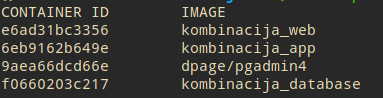
\includegraphics[scale=1]{figures/2-ps.PNG}
					\centering
					\caption{docker ps}
					\label{fig:sekv-uc13}
				\end{figure}
						
				
				
				
		\noindent {\textbf{Dodatna konfiguracija database servisa}}		
				
		 \textit{Database/Dockerfile} konfiguracijska datoteka preuzima najnoviju verziju  \textit{PostgreSQL} baze podataka. Kreira početnog korisnika „postgres“ i dodatnog korisnika „kombinacijauser“. Korisnik „kombinacijauser“ je jedini korisnik koji može raditi izmjene u bazi „kombinacijadb“. Sve navedene vrijednosti je moguće promijeniti u  \textit{env datotekama}. Nikakve druge izmjene nisu potrebne jer će svi ostali servisi uspješno primiti nove vrijednosti.

		 \textit{Database servisu} nije moguće pristupiti izvana, izoliran je na unutarnjoj virtualnoj mreži, ali dijeli dodatnu mrežu s  \textit{pgAdminom}. Za slučaj da se to želi izbjeći potrebno je ukloniti tu mrežu (pgadmin-net) iz database servisa u docker-compose.yml datoteci.	
			
			
						
		\begin{figure}[H]
					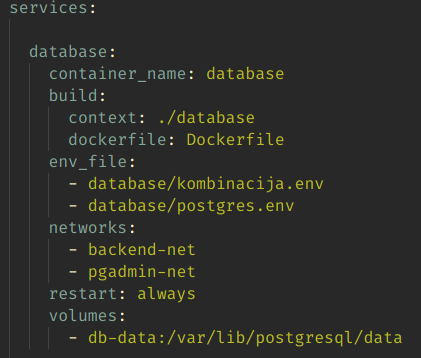
\includegraphics[scale=0.9]{figures/initdb.PNG}
					\centering
					\caption{database networks}
					\label{fig:sekv-uc13}
				\end{figure}
						
			
			
				
		Bazi je moguće pristupiti preko  \textit{pgAdmin servisa} koji je pokrenut na portu  \textit{5000}. Podatci za autentifikaciju na  \textit{pgAdmin} se nalaze u docker-compose.yml datoteci. Podatci za pristup bazi su oni navedeni u  \textit{env datotekama}. Docker ima svoj DNS sustav pa se kao  \textit{hostname} može koristiti ime servisa od baze podataka i interna IP adresa nije potrebna.		
				
		\begin{figure}[H]
					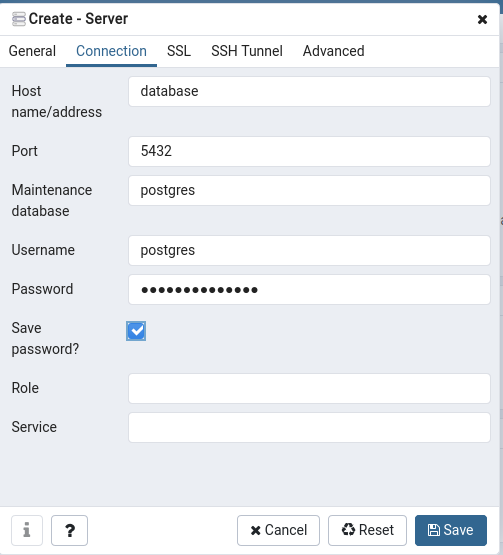
\includegraphics[scale=0.6]{figures/4-pgadmin.PNG}
					\centering
					\caption{pgadmin connect to database}
					\label{fig:sekv-uc13}
				\end{figure} 
												
				
		\noindent {\textbf{Dodatna konfiguracija app servisa}}
		
		 \textit{Backend/Dockerfile} konfiguracijska datoteka preuzima maven 3.6.2 i prevodi Java kod u JAR datoteku. Nakon toga kopira JAR paket u novi servis koji se naziva  \textit{app servis}, a  \textit{maven servis} odbacuje jer više nije potreban. Podatke za spajanje na bazu čita iz  \textit{environment varijabli} koje servisu predaje docker-compose.yml, a čita se iz  \textit{env datoteka} spremljenih u mapi  \textit{database}. U slučaju da su ti podatci prethodno promijenjeni, nije potrebno raditi nikakve izmjene kako u samom izvornom kodu, tako ni u  samim konfiguracijskim datotekama jer će novi biti pročitani pri svakom ponovnom pokretanju.		
		
		\begin{figure}[H]
					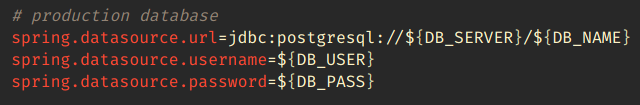
\includegraphics[scale=0.8]{figures/5-env.PNG}
					\centering
					\caption{env app}
					\label{fig:env app}
				\end{figure} 
				
		Za dodatno konfiguriranje Spring-a na serveru potrebno je promijeniti application-prod.properties datoteku jer se ta prenosi u  \textit{app servis} i koristi u produkciji, a obična application.properties datoteka se ignorira. 
Iako se Java aplikacija pokreće na portu  \textit{8080}, taj port nikada neće biti javno dostupan na serveru nego izoliran u Dockeru, a njemu će se pristupati samo unutar sustava preko web servisa koji ima definiran  \textit{proxy} specijalno za tu ulogu.

		Pri prvom pokretanju svi članovi tima se dodaju u bazu kao administratori.\\
		
		
		\noindent {\textbf{Dodatna konfiguracija web servisa}}
		
		 \textit{Frontend/Dockerfile}  konfiguracijska datoteka preuzima najnoviju verziju  \textit{Nginx-a}, kopira mapu  \textit{frontend/public} u  \textit{Nginx} poslužiteljsku mapu kako bi HTML stranice bile javno dostupne, kopira napravljenu  \textit{Nginx konfiguraciju}, namješta domenu servera koju čita iz  \textit{env varijable} (ovu varijablu je potrebno promijeniti), otvara portove  \textit{80} i  \textit{443} na kojima web poslužitelj sluša te time stvara  \textit{Docker web servis} na koji se primaju zahtjevi.

		 \textit{Nginx} konfiguracija se nalazi u datoteci frontend/Nginx/kombinacija.conf. U njoj je na početku definiran  \textit{load balancer} koji vodi na  \textit{app servis (backend)}. U  \textit{load balanceru} se trenutno nalazi samo jedan redak jer postoji samo jedna replika  \textit{app servisa}.  \textit{RR algoritam} je zamijenjen preusmjeravanjem na servis s najmanje aktivnih konekcija.
		
		\begin{figure}[H]
					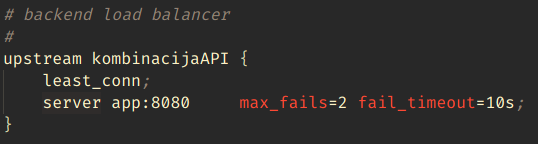
\includegraphics[scale=0.8]{figures/6-load-balancer.PNG}
					\centering
					\caption{load-balancer}
					\label{fig:load-balancer}
				\end{figure} 
		
		Za  \textit{Nginx} su napravljena pravila za cache kako bi se uštedio bandwidth na poslužitelju i smanjila veličina podataka koja se prenosi. Datoteke se čuvaju u web pregledniku klijenata više dana, ali se aktivno provjerava odgovaraju li onima na poslužitelju kako nijedan klijent ne bi imao zastarjelu verziju web stranice.
		
		Naveden je put do SSL certifikata i pravila koja preusmjeravaju korisnike s HTTP-a na HTTPS. Certifikat je generiran  \textit{LetsEncrypt certbot-om}. Putanju do certifikata je potrebno promijeniti ukoliko bi se mijenjao certifikat i lokacija istoga.\\
		
		\noindent {\textbf{MINIMALNI ZAHTJEVI ZA POKRETANJE}}
		
		Aplikacija je pokrenuta na VPS poslužitelju na kojem je instaliran Cent OS 8 Linux. Poslužitelj ima 500 MB RAM memorije, 500 MB SWAP memorije, 5 GB SSD memorije i jednu virtualnu jezgru Intel Xeon procesora (točan broj modela nije otkriven od strane hosting kompanije). To su ujedno i minimalni zahtjevi za pokretanje aplikacije i svih servisa o kojima ovisi. Važno je primijetiti da su to zahtjevi za pokretanje, a ne puštanje u pogon gdje se očekuje veći broj klijenata!
		
		\begin{figure}[H]
					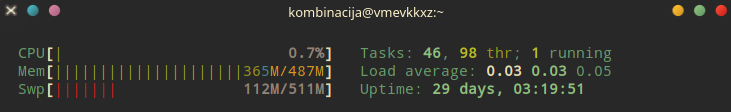
\includegraphics[scale=0.8]{figures/7-htop.PNG}
					\centering
					\caption{htop}
					\label{fig:htop}
				\end{figure} 
		
		\eject 